\documentclass{beamer}
\usepackage{tikz}
\usepackage{graphicx}
\usetikzlibrary{positioning}
%\usetikzlibrary{arrows}

\usefonttheme{professionalfonts}
\usetheme{Boadilla}
\setbeamertemplate{navigation symbols}{}%remove navigation symbols
\hypersetup{pdfstartview={Fit}} % fits the presentation to the window when first displayed
\graphicspath{{./figures/}{./figures/generated/}{./figures/static/}}

%Edwards PB, Wanjura WJ, Brown WV: Selective herbivory by Christmas beetles in response to intraspecific variation in Eucalyptus terpenoids. Oecologia 1993, 95:551–557

%Info
\title[Detecting Somatic Mutations]{Methods for Detecting Somatic Mutation in Plants}
\titlegraphic{
	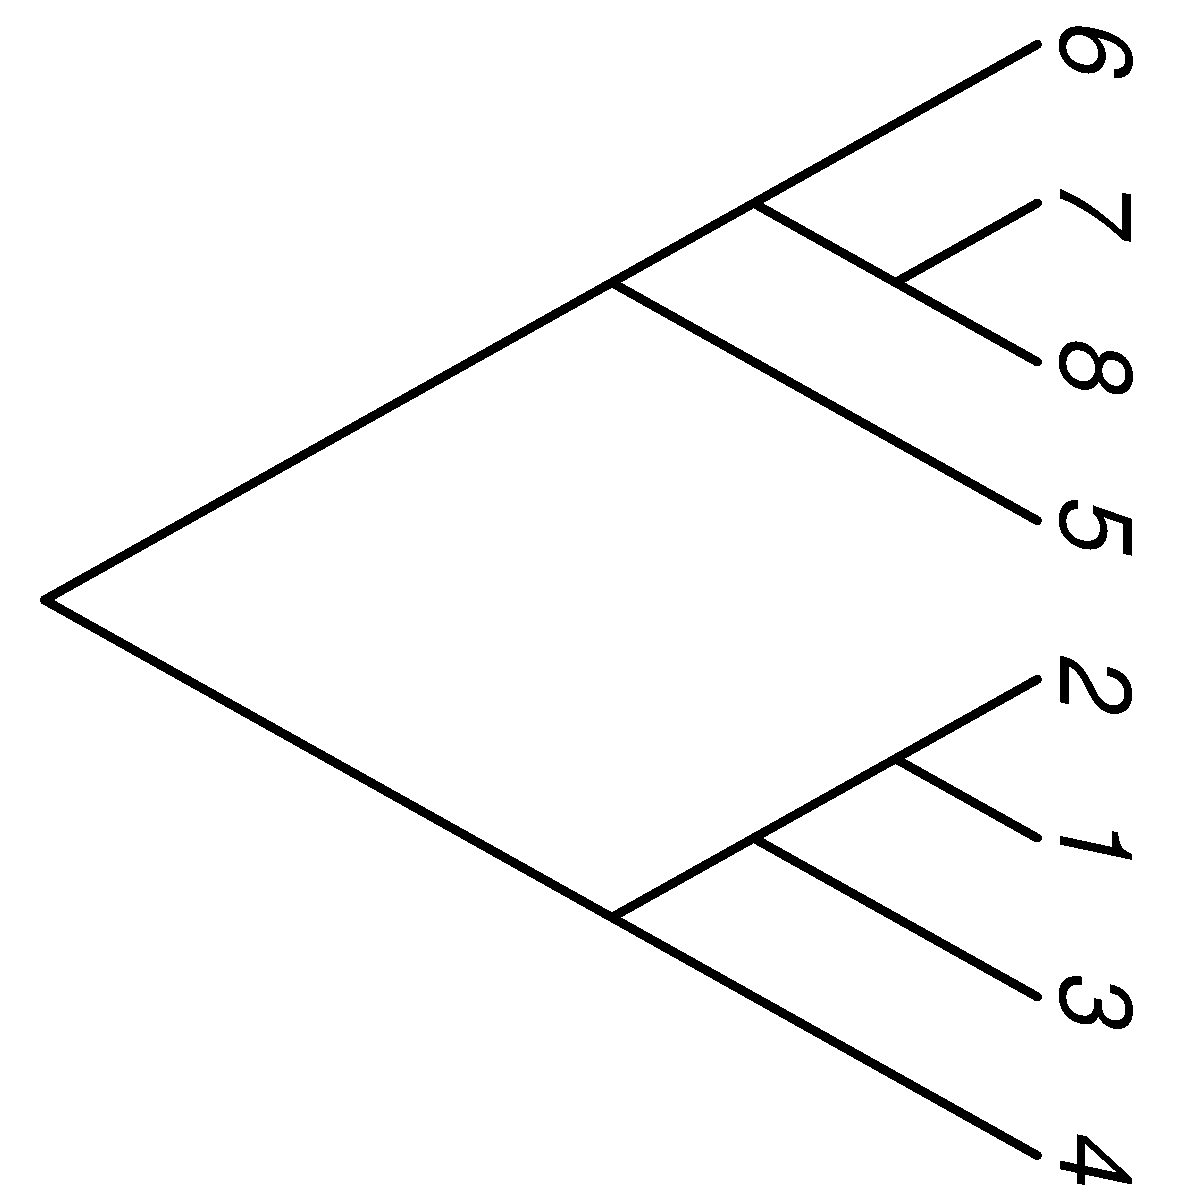
\includegraphics[width=.3\linewidth]{gatk_tree_rightwards.pdf}
	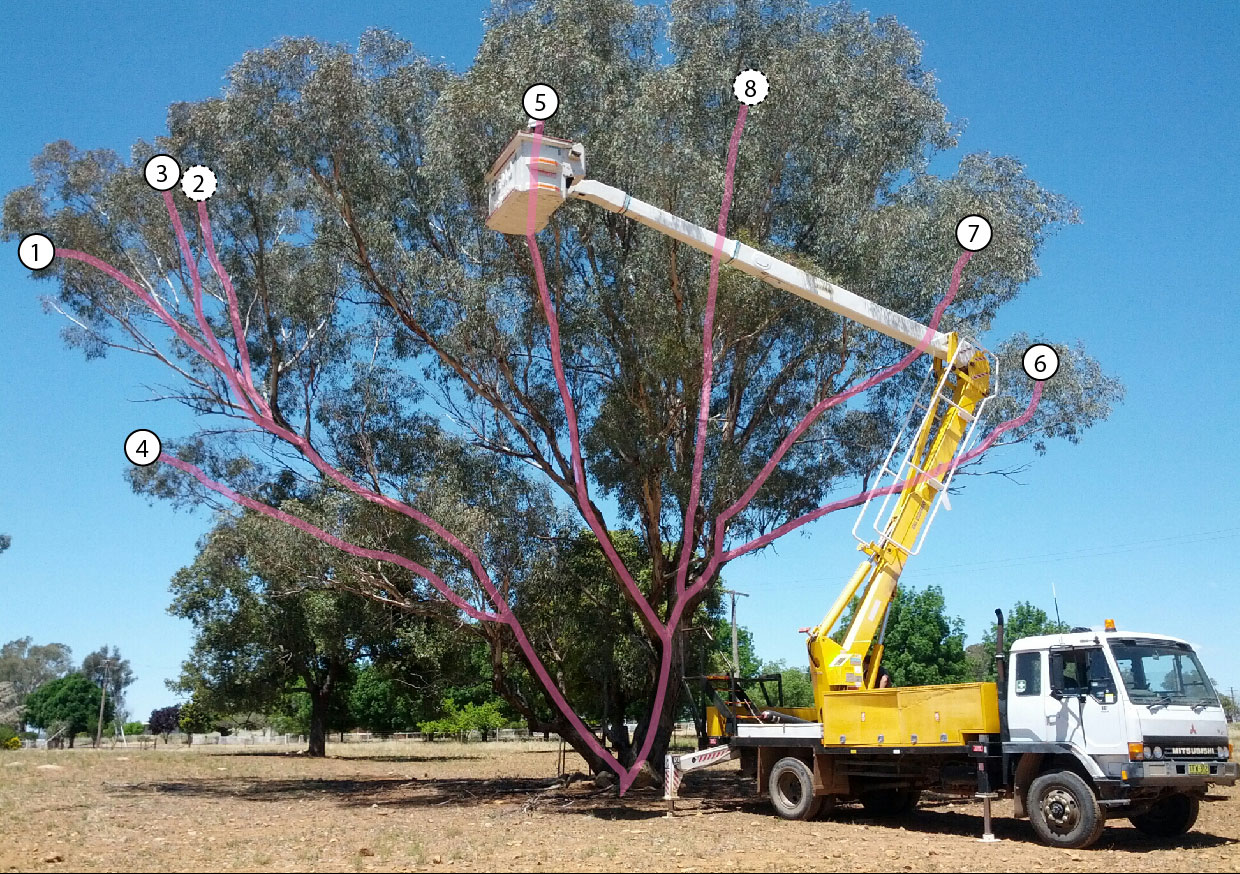
\includegraphics[width=.3\textwidth, angle=90]{labeled_tree.jpg}
	}
\date{3/15/17}
\author{Adam Orr}

\begin{document}
\frame{\titlepage}
\begin{frame}{The Yellow Box Tree: \textit{Eucalyptus melliodora}}

\begin{columns}
\column{.5\linewidth}
\begin{itemize}
\item Produces \textbf{5 times} more nectar than smaller trees.
\item Food source for bees
\item Strong wood used for bridges
\end{itemize}
\column{.5\linewidth}
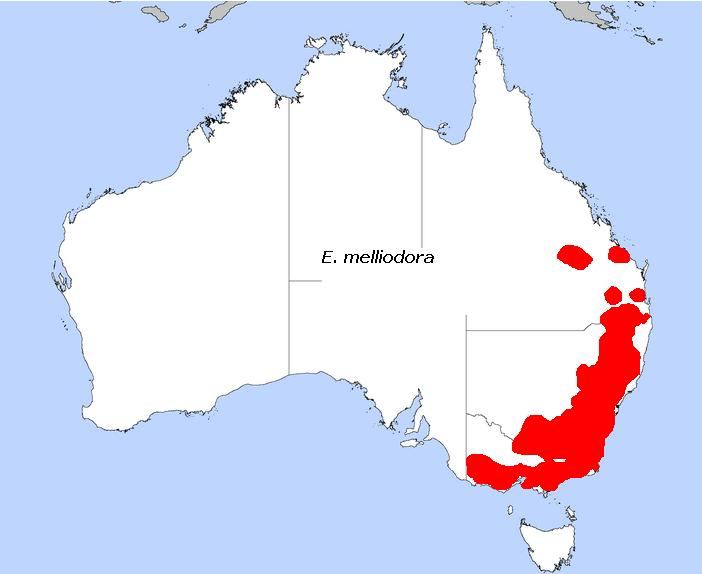
\includegraphics[width=\linewidth]{map.jpg}\footnotemark
\end{columns}
\footnotetext{\url{https://commons.wikimedia.org/wiki/File:E._melliodora.JPG}}
\end{frame}

\begin{frame}{A Genetic Mosaic}
	\begin{center}
	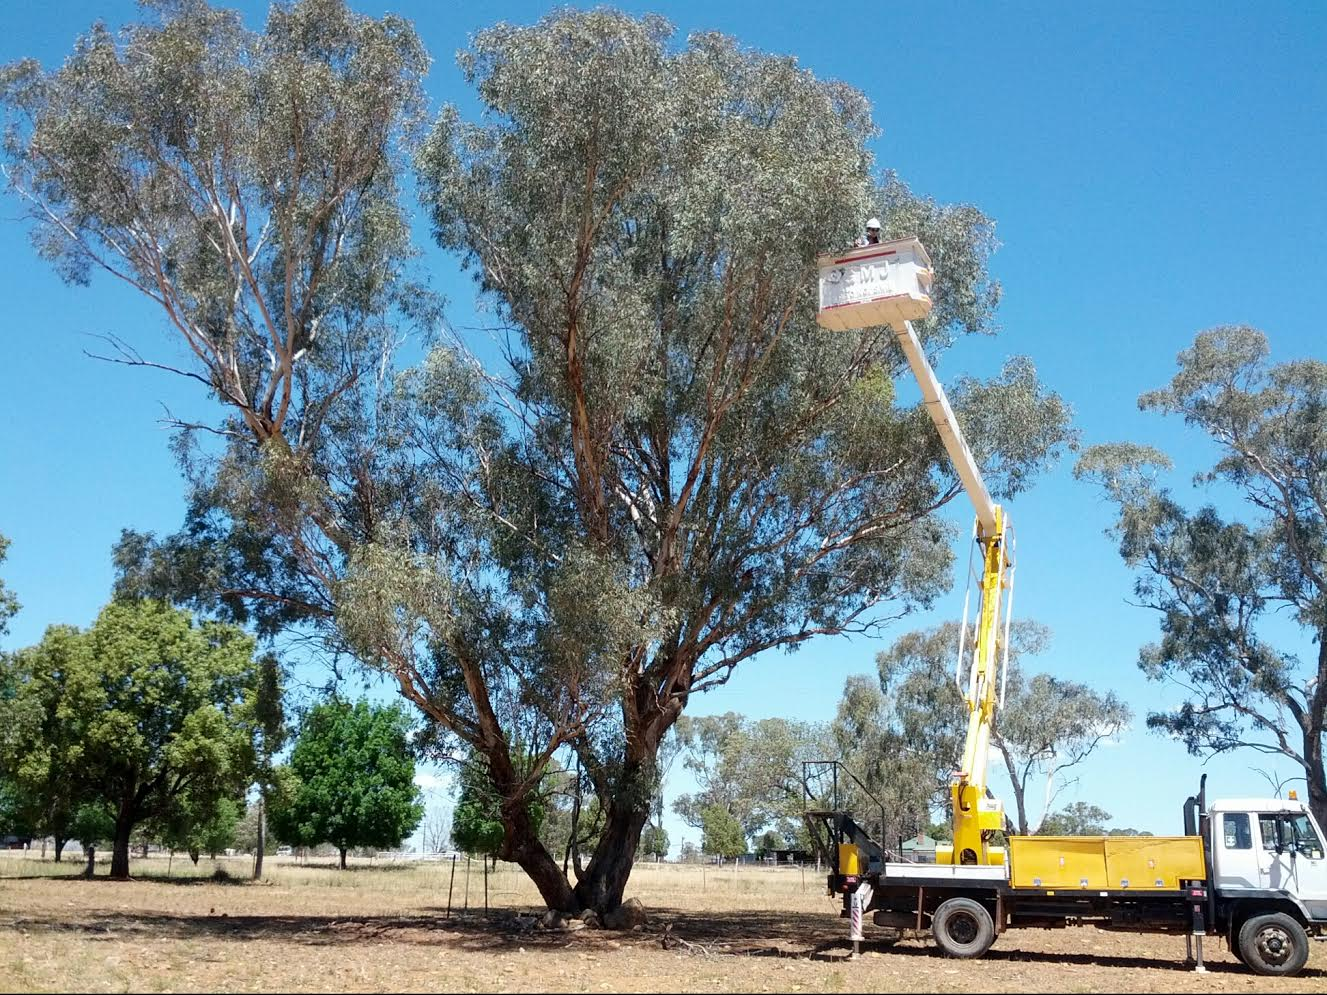
\includegraphics[width=.6\linewidth]{unlabeled_tree.jpg}
	\end{center}
	\begin{itemize}
		\item Edwards identified as mosaic in 1993\footnote{\textit{Edwards PB, Wanjura WJ, Brown WV. Oecologia 1993, 95:551–557.}}
		\item Sheep pen in Yeoval, New South Wales
		\item Differential oil production gives protection from Christmas beetles
		\item Is this mutation a controlled process?
	\end{itemize}
\end{frame}

\begin{frame}{Somatic Mutations are Commercially Interesting}
	\begin{definition}
		A \textbf{somatic mutation} is a mutation that occurs in non-germline cells	
	\end{definition}
	\begin{itemize}
		\item Nectarines arose from a somatic mutation on a peach tree %mosaicism in plants is commercially interesting, though we don't understand it
		\item In botany, this is called a \textbf{sport}
		\item Limited understanding of how plants grow
	\end{itemize}
	\begin{center}
	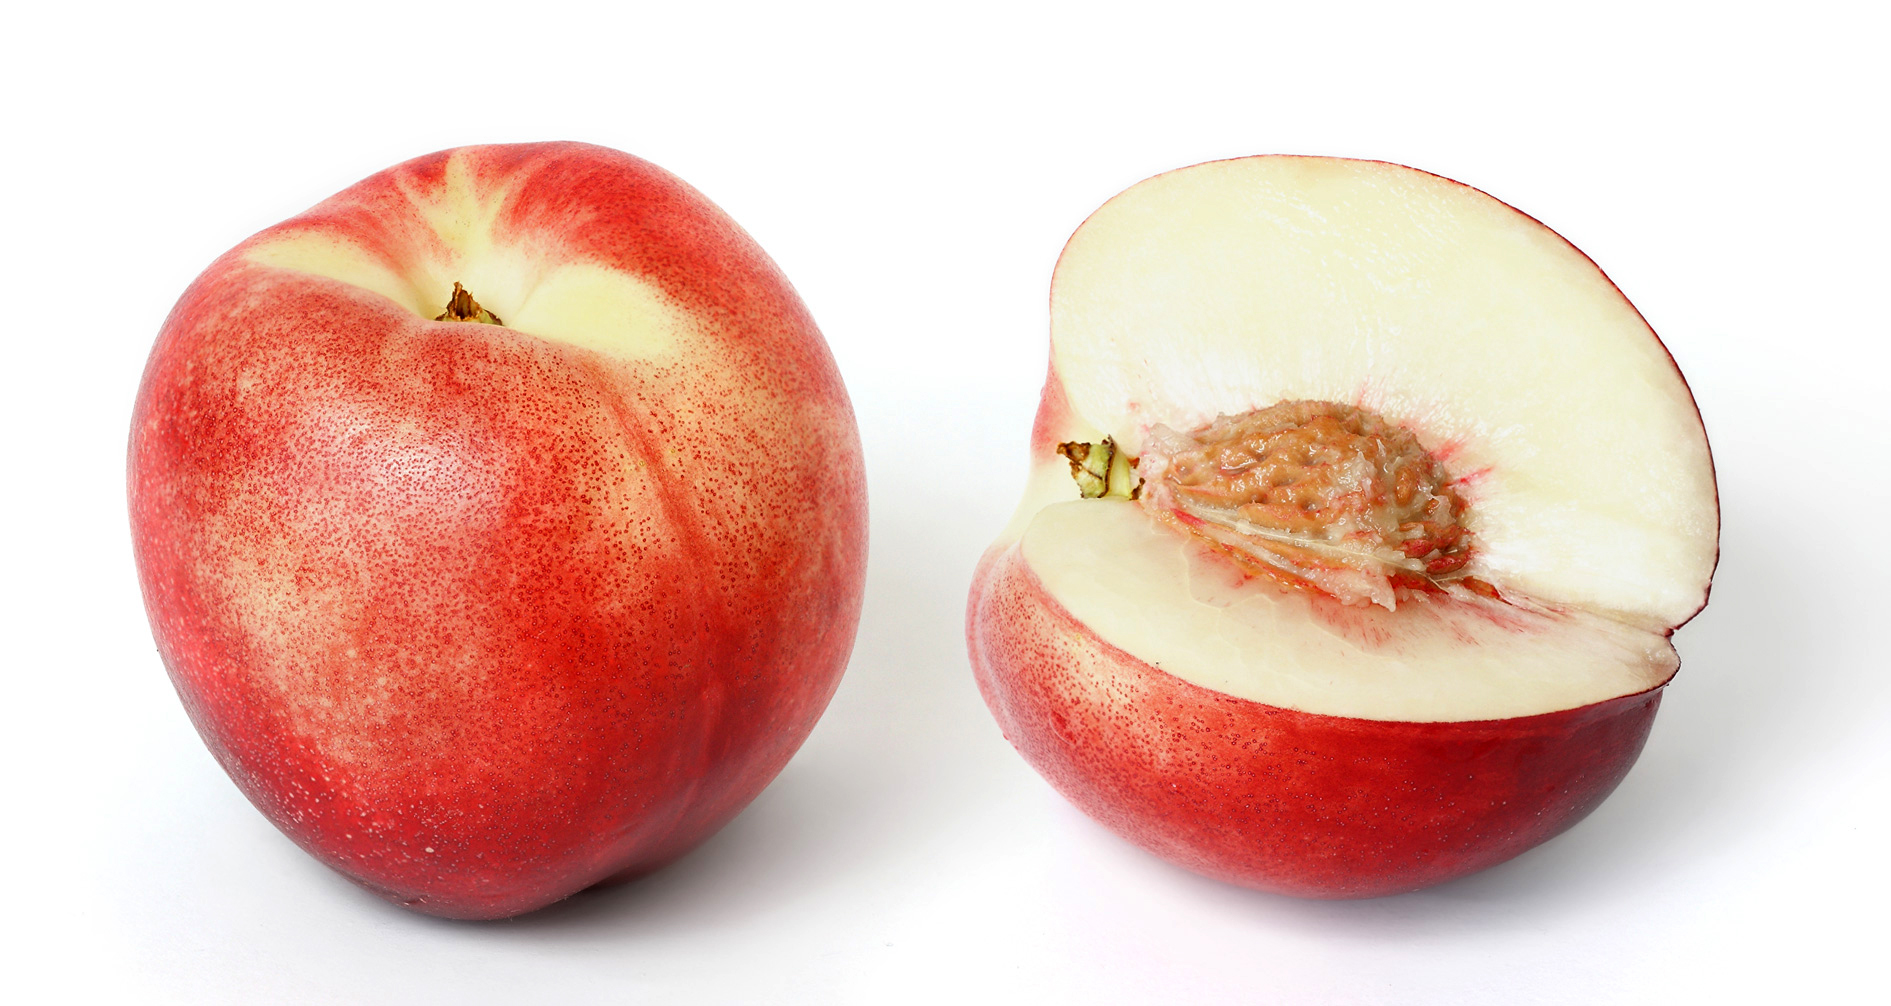
\includegraphics[width=.6\linewidth]{nectarine.jpg}
	\footnote{\url{https://commons.wikimedia.org/wiki/File:White_nectarine_and_cross_section02_edit.jpg}}
	\end{center}
\end{frame}

\begin{frame}{Broad Implications}
	\begin{itemize}
	\item How do somatic mutations spread? How can we study this?
	\item Cancers and other somatic diseases.
	\item A tree as a system for studying somatic mutation.
	\item The tree has a built-in control
	\end{itemize}

	% \begin{alertblock}{A phylogeny is a \textbf{hypothesis}!}
	% 	We use simulations because we can't know the truth \\~\\

	% 	Knowing the truth will allow us to evaluate phylogenetic tools		
	% \end{alertblock}

\end{frame}

\begin{frame}{What mutation is causing the herbivore resistance phenotype?}
\begin{center}
	\begin{tikzpicture}
		\node[anchor=south west,inner sep=0] (image) at (0,0) {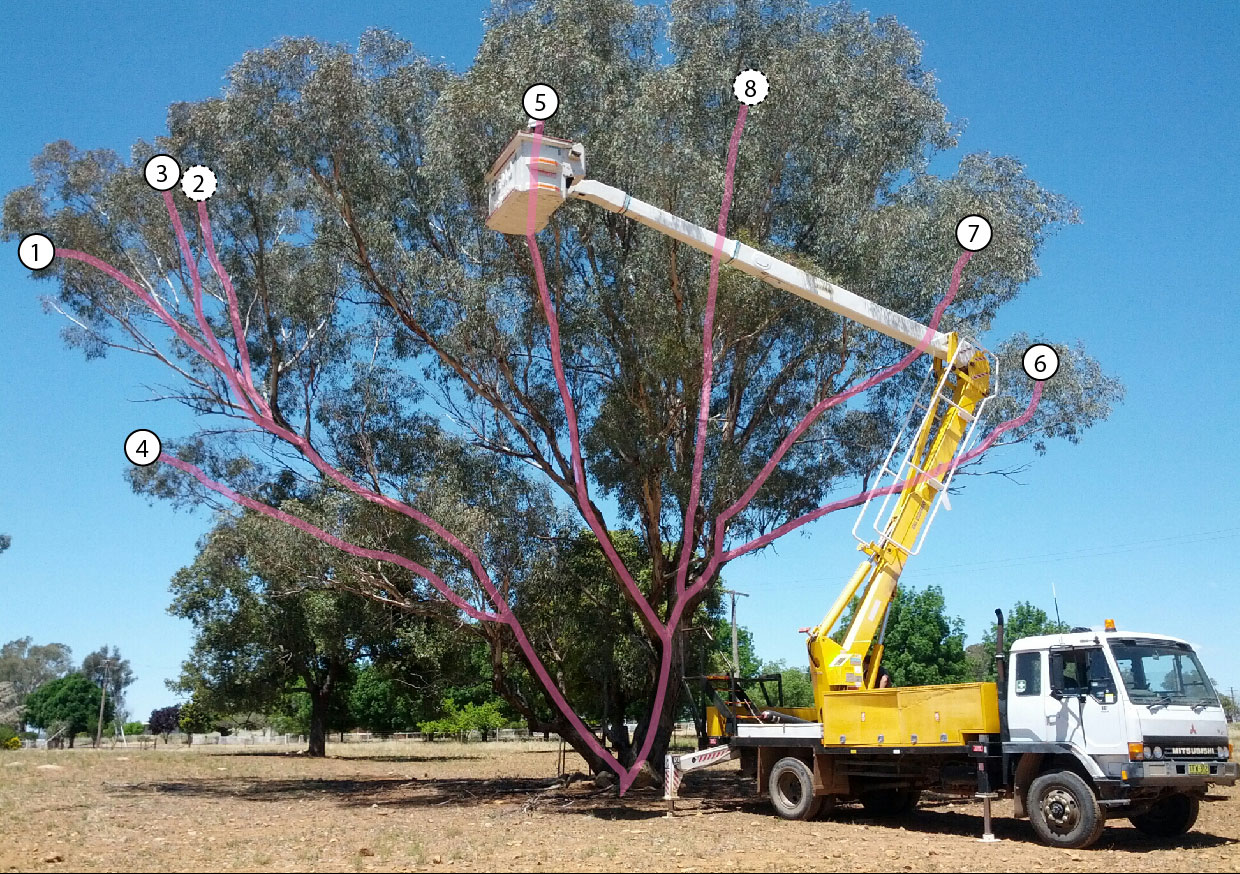
\includegraphics[width=\textwidth]{labeled_tree.jpg}};
		\begin{scope}[x={(image.south east)},y={(image.north west)}]
			\draw[red, line width=5mm, ->] (.35,.75) -- (.25,.5);
		\end{scope}
	\end{tikzpicture}
\end{center}
\end{frame}


%%A slide about cancer. Can we extract all the populations out of a tumor? Can we use a sequencing strategy to identify human GT vs cancer GT?

%%We believe it to be the case that flowers & reproductive cells are forming as the branch forms, not transported through a stem-cell store.

\begin{frame}{Mutations are very rare, but sequencing errors are very common.}

Somatic mutations are hard to find

\begin{itemize}
\item Errors accumulate during PCR prior to sequencing - then propagate
\item Errors accumulate in amplification steps during sequencing
\item Technical error from sequencer
\end{itemize}

\textbf{Sequencing error} alone is \textbf{$\sim10^{-2}$} while mutation rate after error-checking is \textbf{$\sim10^{-10}$}

\end{frame}

\begin{frame}{Study Methodology}
\begin{columns}

\column{.5\linewidth}
\begin{definition}
\textbf{Coverage:}Average number of times a single base is sequenced.
\end{definition}
\begin{itemize}
\item Sequence 8 samples in triplicate
\item Ultra-deep coverage for each replicate ($\sim$30X)
\item Align sequence to genome of \textit{Eucalyptus grandis}
\item Use replicates to remove false positives
\end{itemize}

\column{.5\linewidth}
\begin{center}
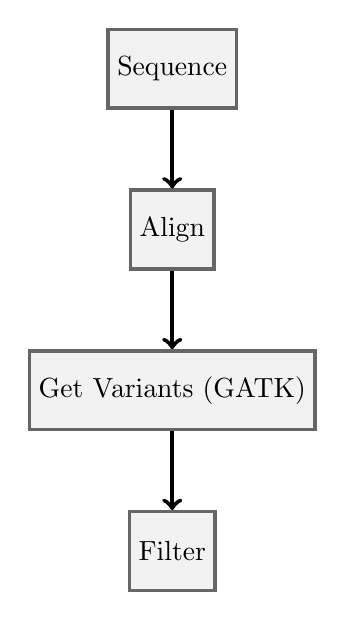
\begin{tikzpicture}[sqnode/.style={rectangle, draw=black!60, fill=black!5,very thick,minimum size=1cm}]
	\node[sqnode] (sequencing) {Sequence};
	\node[sqnode] (alignment) [below = of sequencing] {Align};
	\node[sqnode] (varcall) [below = of alignment] {Get Variants (GATK)};
	\node[sqnode] (flt) [below = of varcall] {Filter};
	\draw[ultra thick,->] (sequencing.south) -- (alignment.north);
	\draw[ultra thick,->] (alignment.south) -- (varcall.north);
	\draw[ultra thick,->] (varcall.south) -- (flt.north);
\end{tikzpicture}
\end{center}
\end{columns}
\end{frame}

%TODO: Need a sideways tree, a dendogram, and a normal tree

\begin{frame}{Mutation Pattern Approximately Matches Tree Structure}
\begin{columns}
\column{.5\linewidth}
	\begin{center}
	Computed Tree
	\end{center}
	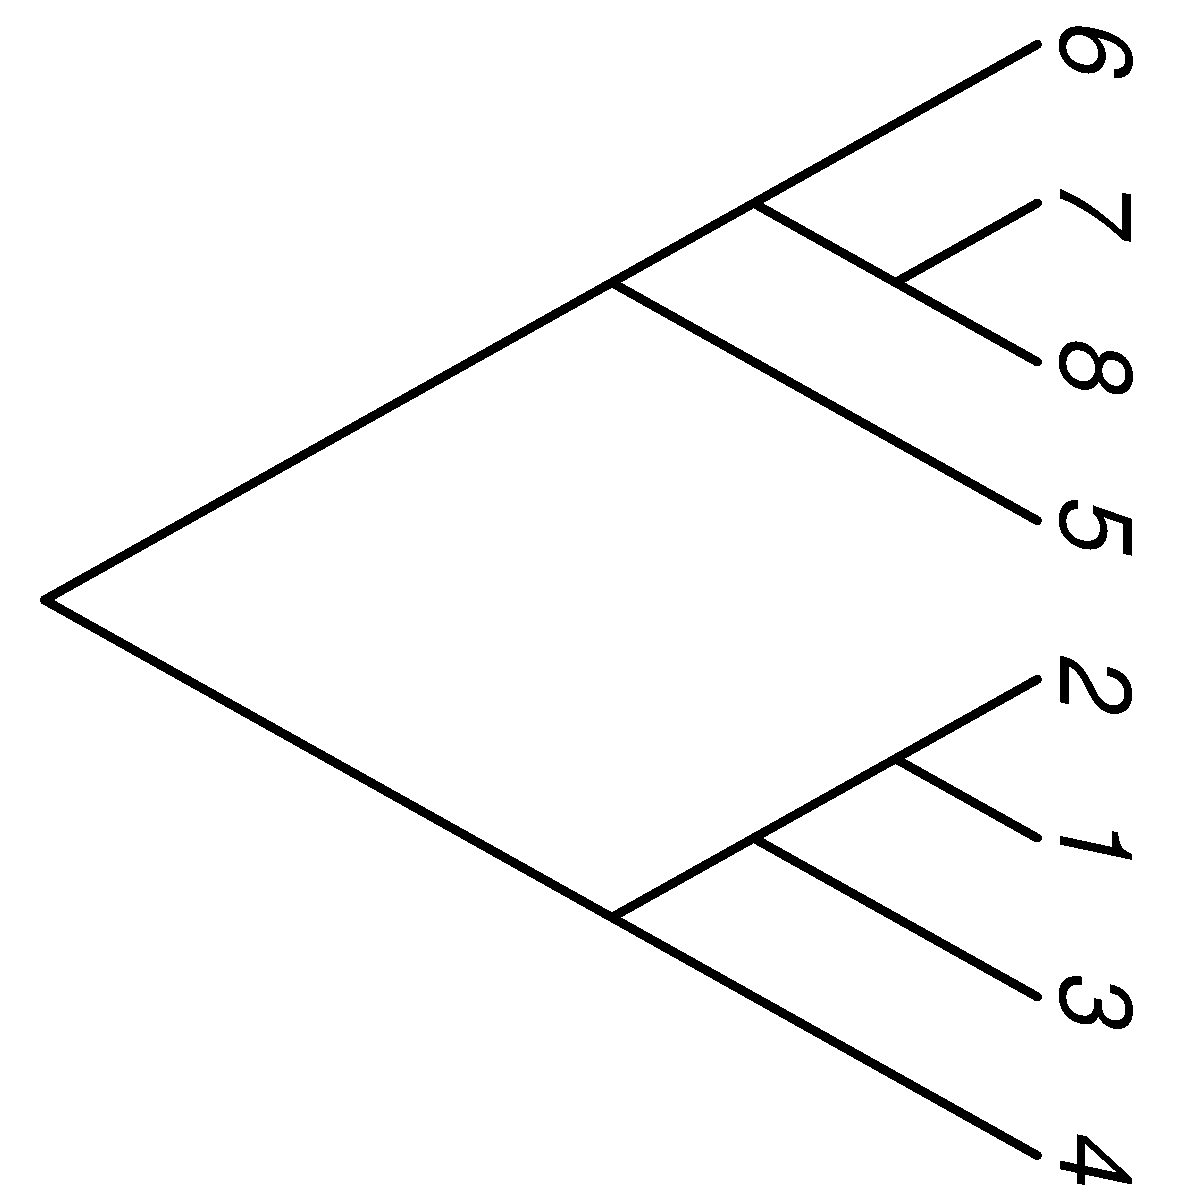
\includegraphics[width=\linewidth]{gatk_tree_rightwards.pdf}
\column{.5\linewidth}
	\begin{center}
	True Tree
	\end{center}
	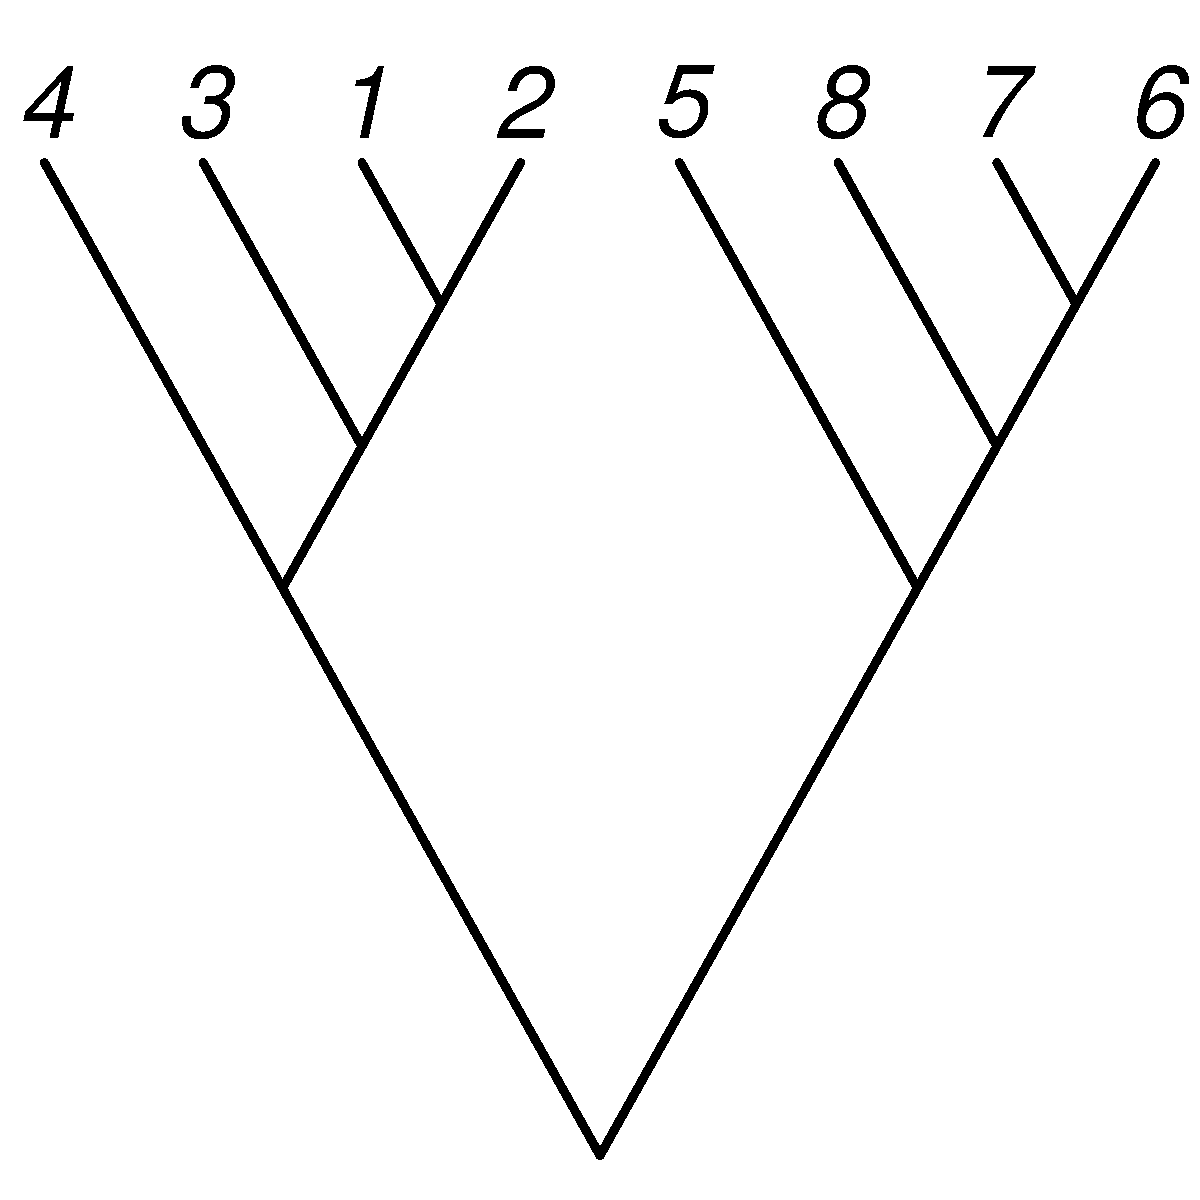
\includegraphics[width=\linewidth,angle=90]{true_tree.pdf}
\end{columns}
\end{frame}

\begin{frame}{Most Reads Are Not Mapped to the \textit{E. grandis} Reference}
\begin{center}
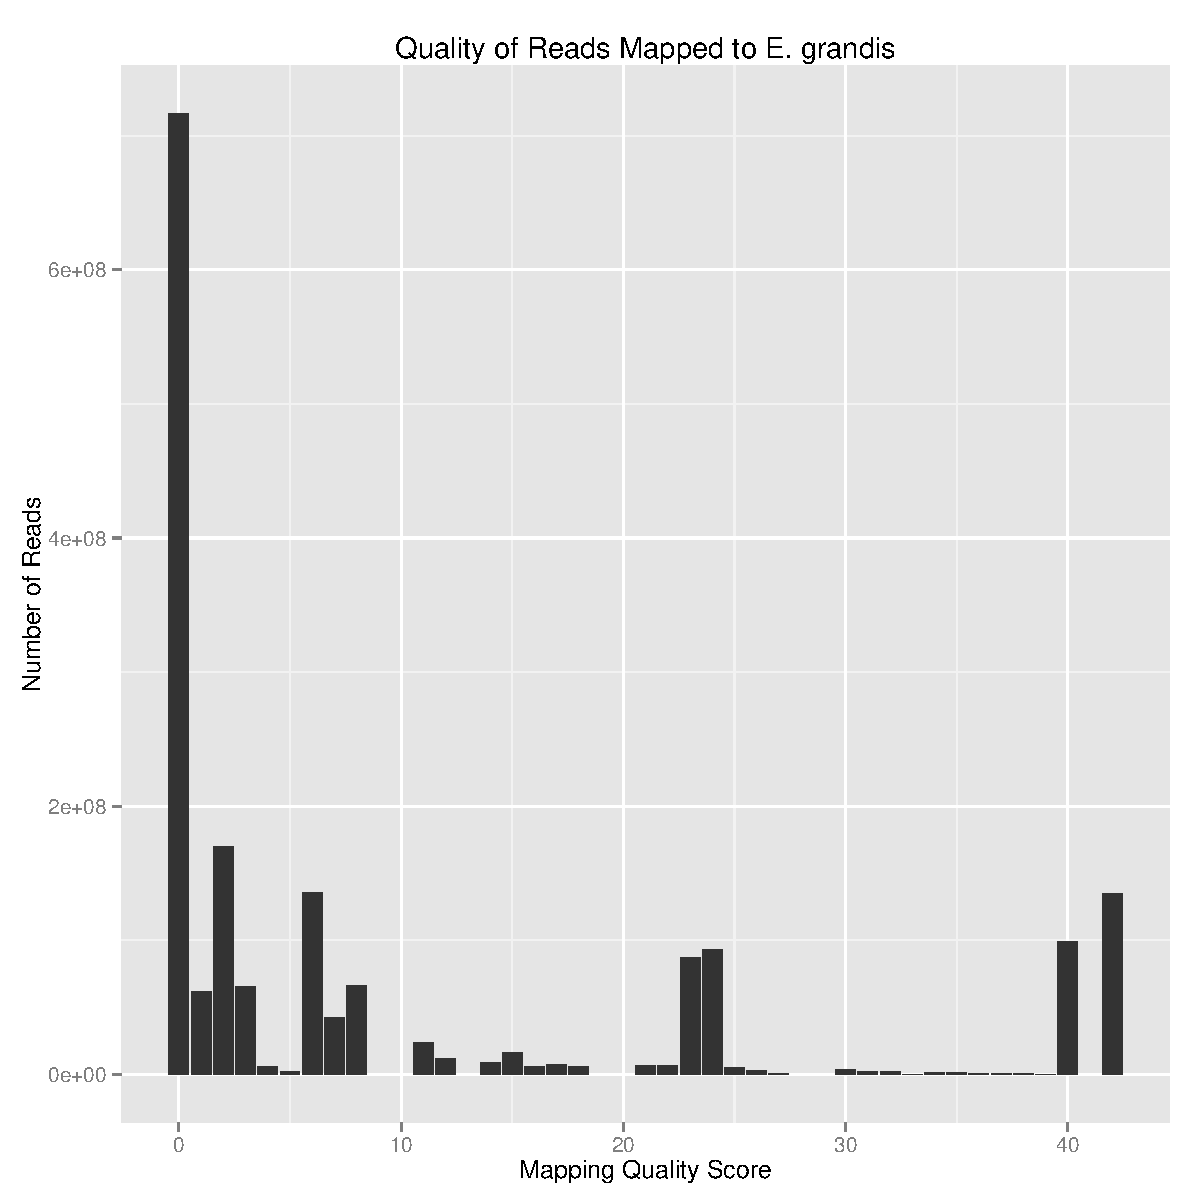
\includegraphics[width=\linewidth]{bowtie1_hist.pdf}
\end{center}
\end{frame}

\begin{frame}{A Reference-Free Method}
\begin{columns}
\column{.5\linewidth}
\begin{center}
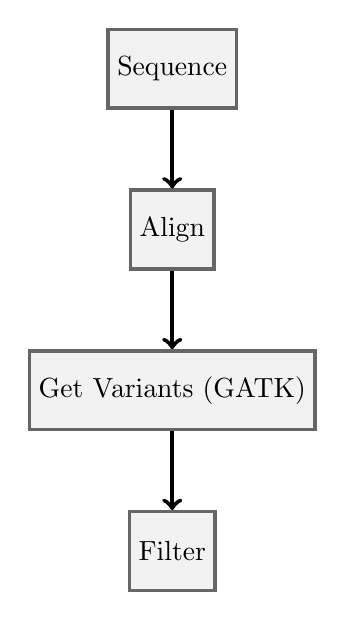
\begin{tikzpicture}[sqnode/.style={rectangle, draw=black!60, fill=black!5,very thick,minimum size=1cm}]
	\node[sqnode] (sequencing) {Sequence};
	\node[sqnode] (alignment) [below = of sequencing] {Align};
	\node[sqnode] (varcall) [below = of alignment] {Get Variants (GATK)};
	\node[sqnode] (flt) [below = of varcall] {Filter};
	\draw[ultra thick,->] (sequencing.south) -- (alignment.north);
	\draw[ultra thick,->] (alignment.south) -- (varcall.north);
	\draw[ultra thick,->] (varcall.south) -- (flt.north);
\end{tikzpicture}
\end{center}
\column{.5\linewidth}
\begin{center}
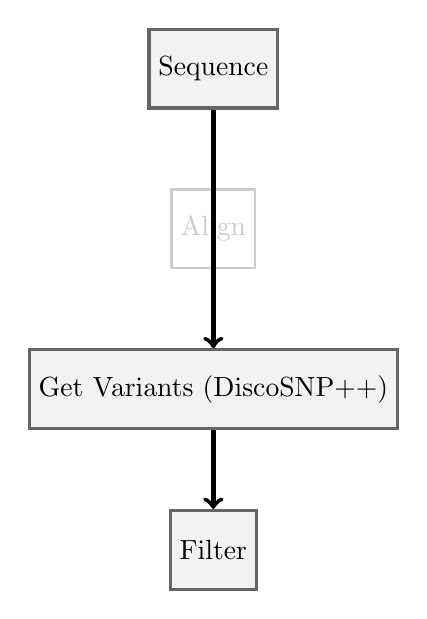
\begin{tikzpicture}[sqnode/.style={rectangle, draw=black!60, fill=black!5,very thick,minimum size=1cm}, gnode/.style={rectangle, text=black!20, draw = black!20, thick, minimum size=1cm}]
	\node[sqnode] (sequencing) {Sequence};
	\node[gnode] (alignment) [below = of sequencing] {Align};
	\node[sqnode] (varcall) [below = of alignment] {Get Variants (DiscoSNP++)};
	\node[sqnode] (flt) [below = of varcall] {Filter};
	\draw[ultra thick,->] (sequencing.south) -- (varcall);
	\draw[ultra thick,->] (varcall.south) -- (flt.north);
\end{tikzpicture}
\end{center}
\end{columns}
\end{frame}

% \begin{frame}{Illumina Library Preparation}
% 	\begin{columns}
% 		\column{.5\linewidth}
% 			\begin{itemize}
% 			\item The advantage of Illumina: massive parallelization
% 			\item Amplify your DNA
% 			\item \textbf{Physically} shear your DNA
% 			\item Add adaptors and inserts to your DNA fragments
% 			\end{itemize}
% 		\column{.5\linewidth}
% 			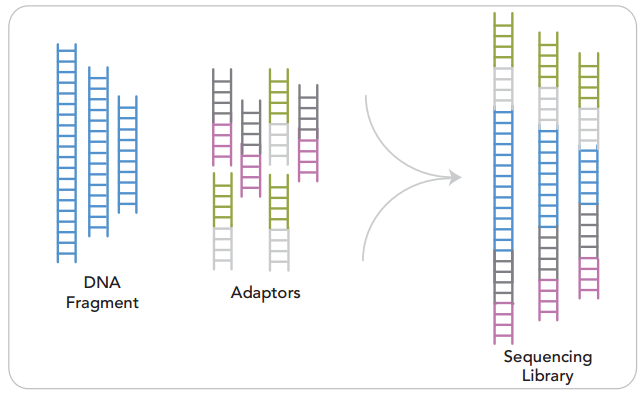
\includegraphics[width=\linewidth]{illumina_library_prep.png}
% 	\end{columns}
% \end{frame}

% \begin{frame}{Illumina Sequencing}
% 	\begin{columns}
% 		\column{.5\linewidth}
% 			\begin{itemize}
% 			\item Adaptor is bound to chip
% 			\item Bridge amplification
% 			\item Both strands are bound to chip
% 			\item Flood with fluorescent nucleotides
% 			\item Rinse and repeat
% 			\end{itemize}
% 			\begin{block}{Smile for the Camera}
% 			Illumina sequencing is a problem of optics. Advances in Illumina sequencing are all fundamentally advances in camera technology. 
% 			\end{block}
% 		\column{.5\linewidth}
% 			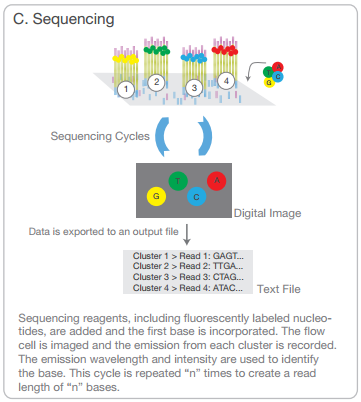
\includegraphics[width=\linewidth]{sequencing.png}
% 	\end{columns}
% \end{frame}

% \begin{frame}{Assembly}
% 	\begin{definition}
% 	A \textbf{contig} is a contiguous stretch of sequence that has been assembled from reads.
% 	\end{definition}

% 	\begin{itemize}
% 	\item Look for overlaps between sequence
% 	\item Long contig lengths is a sign of a good assembly
% 	\item Very computationally expensive and time-consuming
% 	\item Difficult to get right
% 	\item Contigs are \textbf{not} chromosomes
% 	\item Sometimes transcript data can be used to join contigs
% 	\end{itemize}
% \end{frame}

% \begin{frame}{Alignment}
% 	\begin{definition}
% 	A \textbf{read} is a short (150ish bp) segment of sequence determined by the sequencer.
% 	\end{definition}

% 	\begin{itemize}
% 	\item Line up reads to a reference
% 	\item Some software takes advantage of paired-end technology to improve alignment
% 	\end{itemize}
% 	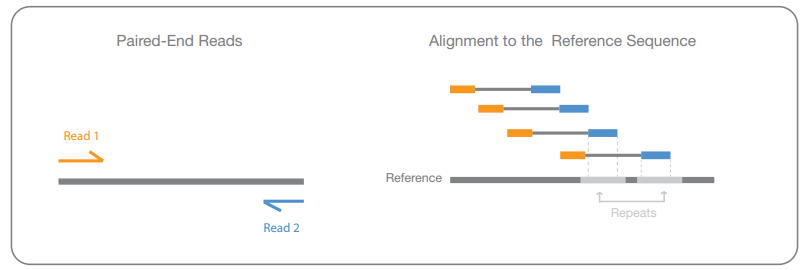
\includegraphics[width=\linewidth]{pe_sequencing.png}
% \end{frame}



% \begin{frame}{Variant Calling}
% 	\begin{definition}
% 	\textbf{Coverage} is the number of reads aligned at a particular position. Large variations in coverage is a symptom of poor alignment or library prep. 
% 	\end{definition}

% 	\begin{columns}
% 		\column{.5\linewidth}
% 			\begin{itemize}
% 			\item Account for sequencing error
% 			\item Variation in sequenced population
% 			\item Ploidy
% 			\item Could be complex algorithm, may be as simple as checking if the base agrees with the reference.
% 			\end{itemize}
% 		\column{.5\linewidth}
% 			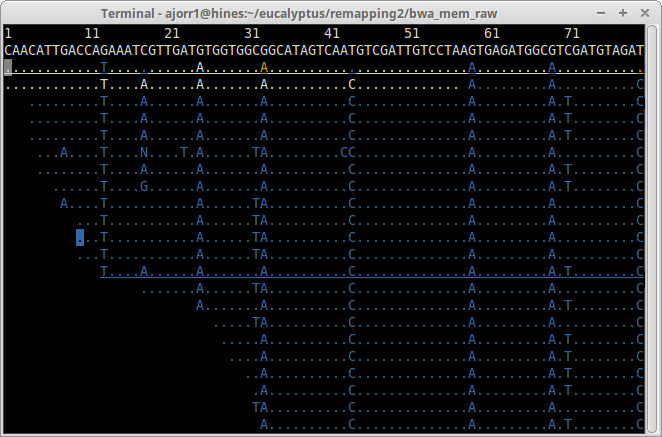
\includegraphics[width=\linewidth]{coverage.png}
% 	\end{columns}
% \end{frame}

% \begin{frame}{The Pipeline}
% 	\begin{alertblock}{No Reference}
% 		If you don't have a reference genome available, all these steps are required to call variants
% 	\end{alertblock}
% 	\vfill
% 	\begin{tikzpicture}[sqnode/.style={circle, draw=black!60, fill=black!5,very thick}]
% 		\node[sqnode] (sequencing) {Sequencing};
% 		\node[sqnode] (assembly) [right=of sequencing] {Assembly};
% 		\node[sqnode] (alignment) [right = of assembly] {Alignment};
% 		\node[sqnode] (varcall) [right = of alignment] {Variant Calling};
% 		\draw[ultra thick,->] (sequencing.east) -- (assembly.west);
% 		\draw[ultra thick,->] (assembly.east) -- (alignment.west);
% 		\draw[ultra thick,->] (alignment.east) -- (varcall.west);
% 	\end{tikzpicture}
% 	\vfill
% \end{frame}

% \begin{frame}{What if there was a better way?}
% 	\begin{tikzpicture}[sqnode/.style={circle, draw=black!60, fill=black!5,very thick},lightnode/.style={circle,draw=black!10,fill=black!2,very thick}]
% 		\node[sqnode] (sequencing) {Sequencing};
% 		\node[lightnode] (assembly) [right=of sequencing] {Assembly};
% 		\node[lightnode] (alignment) [right = of assembly] {Alignment};
% 		\node[sqnode] (varcall) [right = of alignment] {Variant Calling};
% 		%\draw[ultra thick,->] (sequencing.east) -- (assembly.west);
% 		%\draw[ultra thick,->] (assembly.east) -- (alignment.west);
% 		%\draw[ultra thick,->] (alignment.east) -- (varcall.west);
% 		\draw[ultra thick,->] (sequencing.south) .. controls +(down:30mm) and +(down:30mm) .. (varcall.south);
% 	\end{tikzpicture}
% \end{frame}

% \begin{frame}{What is a graph?}
% 	\begin{definition}
% 	A \textbf{graph} is a set of nodes and a set of edges, G = (V,E)
% 	\end{definition}
% 	\centering
% 	\begin{tikzpicture}[cnode/.style={circle, draw = black!60, fill=black!5,very thick, minimum size = 20mm}]
% 		\node[cnode] (leftnd) {1};
% 		\node[cnode] (rightnd) [right = of leftnd]{2};
% 		\draw[very thick] (leftnd.east) -- (rightnd.west);
% 	\end{tikzpicture}

% 	V = \{1 , 2\}

% 	E = \{(1,2)\}

% \end{frame}

\begin{frame}{The De Bruijn Graph}
	\begin{definition}
	A \textbf{De Bruijn Graph} is a graph where the nodes represent symbols and edges represent overlaps between those symbols.
	\end{definition}

	\begin{example}
	\begin{center}
	Consider the sequence \textbf{AATGCAT} and split it with \textbf{kmer} size 3

	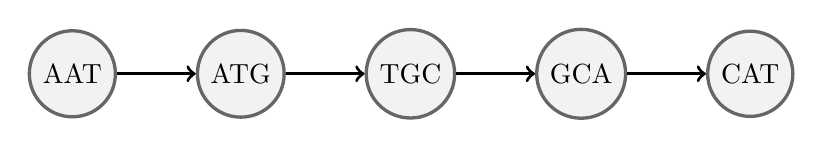
\begin{tikzpicture}[cnode/.style={circle,draw=black!60,fill=black!5,very thick}]
		\node[cnode] (aat) {AAT};
		\node[cnode] (atg) [right = of aat] {ATG};
		\node[cnode] (tgc) [right = of atg] {TGC};
		\node[cnode] (gca) [right = of tgc] {GCA};
		\node[cnode] (cat) [right = of gca] {CAT};
		\draw[very thick,->] (aat.east) -- (atg.west);
		\draw[very thick,->] (atg.east) -- (tgc.west);
		\draw[very thick,->] (tgc.east) -- (gca.west);
		\draw[very thick,->] (gca.east) -- (cat.west);
	\end{tikzpicture}
	\end{center}
	\end{example}

\end{frame}

\begin{frame}{Calling Variants Using Bubbles}

A difference in one base will cause a \textbf{bubble} to form in the graph.

\begin{example}
Consider the sequence \textbf{AATGCAT} and split it with \textbf{kmer} size 3.
There is a sample with a G to C mutation!

\begin{center}
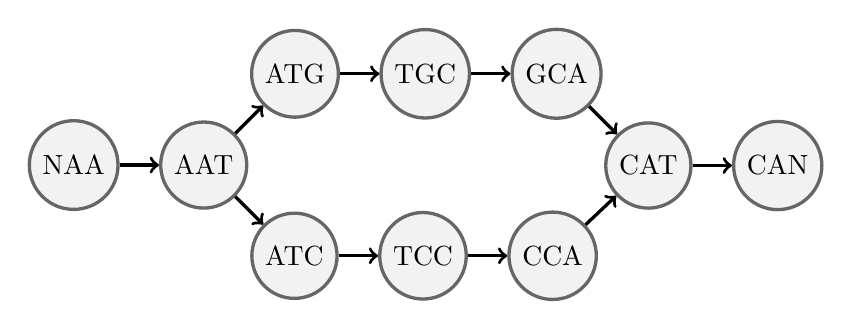
\begin{tikzpicture}[cnode/.style={circle,draw=black!60,fill=black!5,very thick}, node distance = .5 cm]
	\node[cnode] (upstream) {NAA};
	\node[cnode] (aat) [right = of upstream] {AAT};
	\node[cnode] (atg) [above right = of aat] {ATG};
	\node[cnode] (tgc) [right = of atg] {TGC};
	\node[cnode] (gca) [right = of tgc] {GCA};
	\node[cnode] (cat) [below right = of gca] {CAT};
	\node[cnode] (atc) [below right = of aat] {ATC};
	\node[cnode] (tcc) [right = of atc] {TCC};
	\node[cnode] (cca) [right = of tcc] {CCA};
	\node[cnode] (downstream) [right = of cat] {CAN};
	\draw[very thick,->] (upstream) -- (aat);
	\draw[very thick,->] (aat) -- (atg);
	\draw[very thick,->] (atg.east) -- (tgc.west);
	\draw[very thick,->] (tgc.east) -- (gca.west);
	\draw[very thick,->] (gca) -- (cat);
	\draw[very thick,->] (aat) -- (atc);
	\draw[very thick,->] (atc.east) -- (tcc.west);
	\draw[very thick,->] (tcc.east) -- (cca.west);
	\draw[very thick,->] (cca) -- (cat);
	\draw[very thick,->] (cat) -- (downstream);
\end{tikzpicture}
\end{center}
\end{example}

\end{frame}

\begin{frame}{The Reference-Free Method Performs Similarly}
	\begin{columns}
	\column{.5\linewidth}
		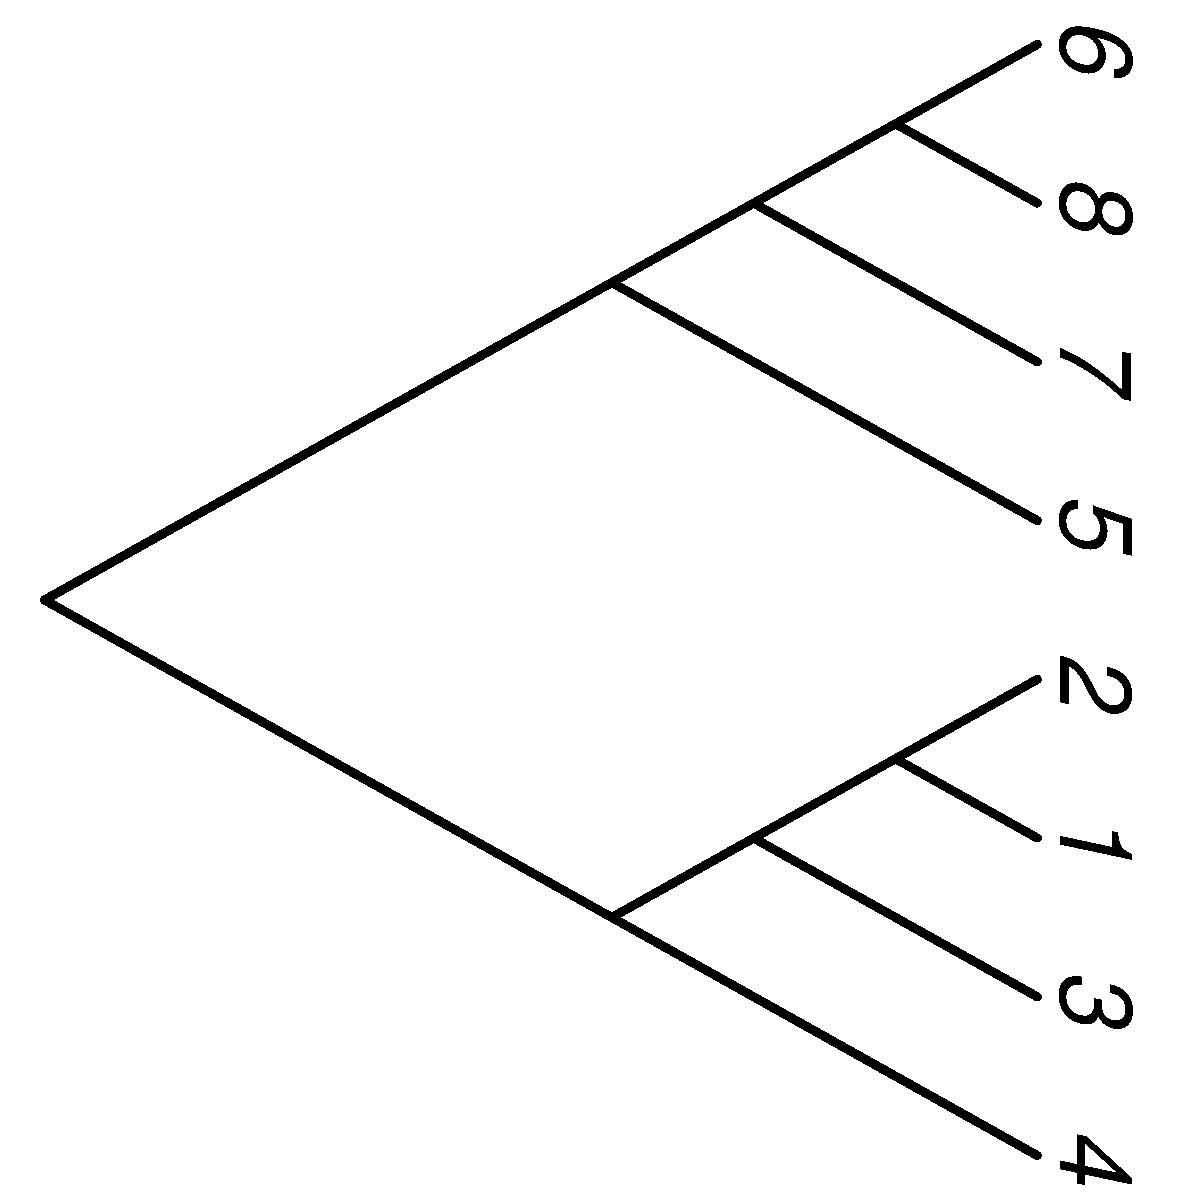
\includegraphics[width=\linewidth]{disco_tree_rightwards.pdf}
	\column{.5\linewidth}
		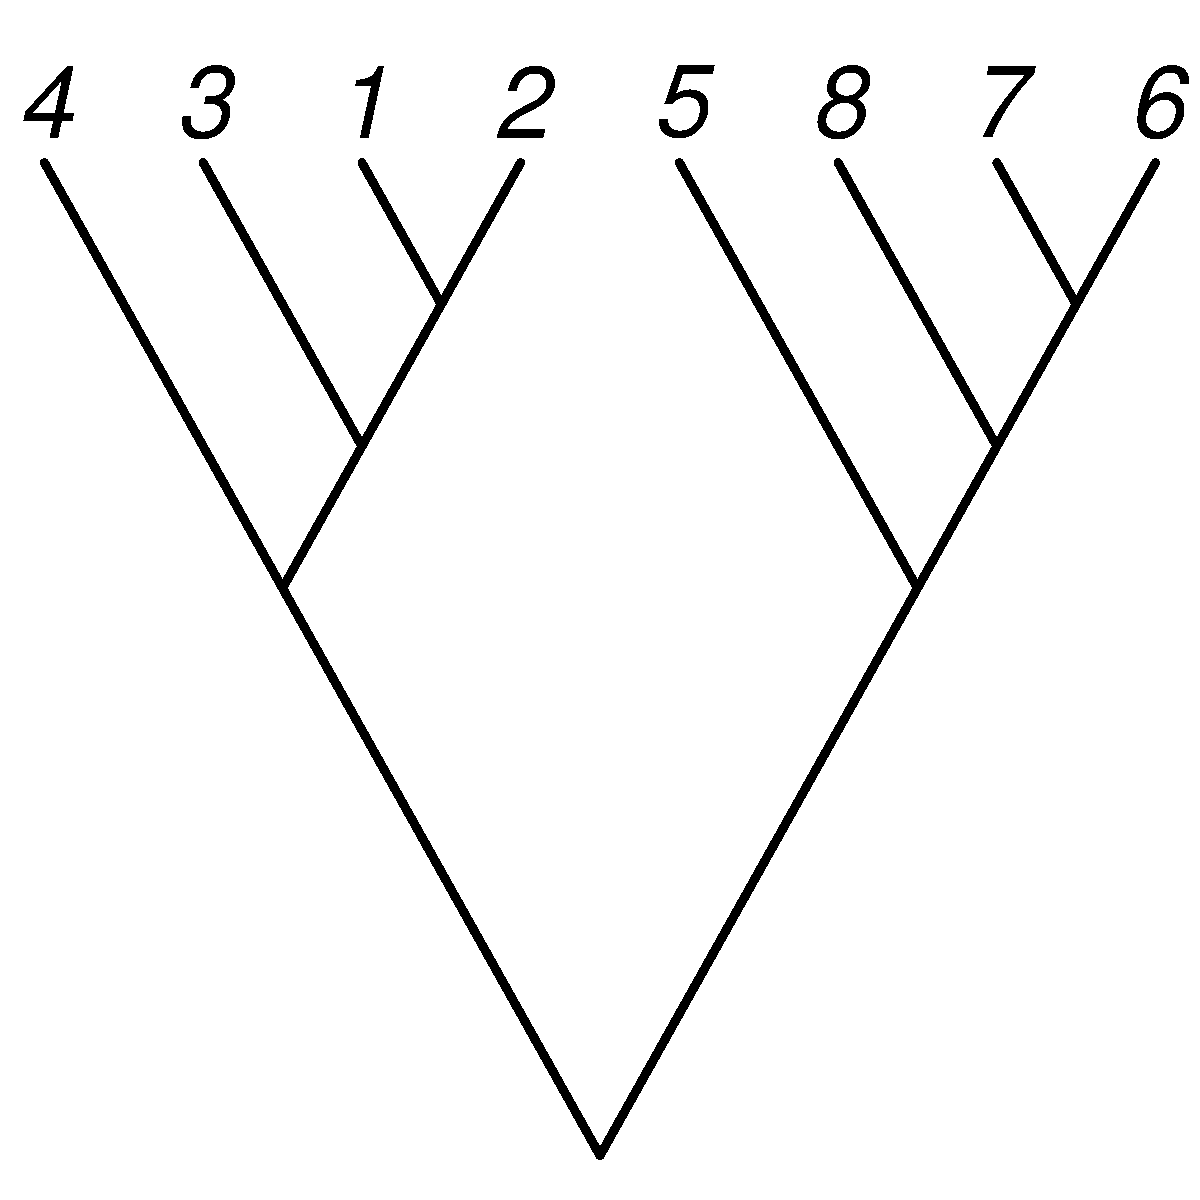
\includegraphics[width=\linewidth,angle=90]{true_tree.pdf}
	\end{columns}
\end{frame}

% \begin{frame}{The Genome Analysis Toolkit}
% 	\begin{itemize}
% 	\item Used a traditional variant-calling pipeline: GATK best practices workflow
% 	\item Reference genome of a close relative: \textit{Eucalyptus Grandis}
% 	\end{itemize}
% 	\begin{columns}
% 	\column{.5\linewidth}
% 		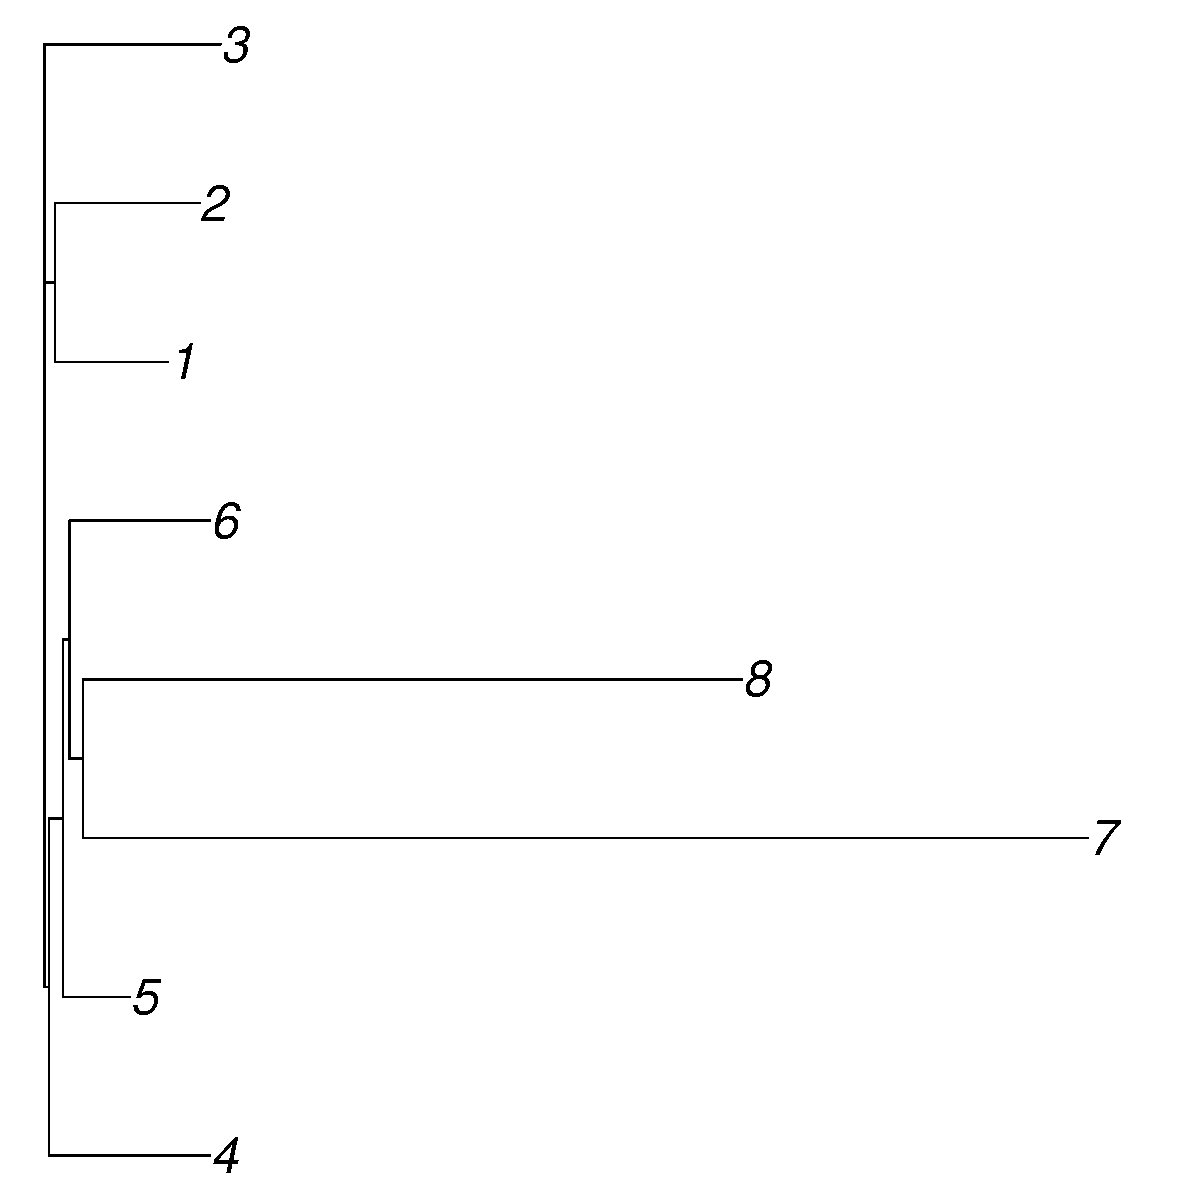
\includegraphics[width=\linewidth]{gatk_tree2.pdf}
% 	\column{.5\linewidth}
% 		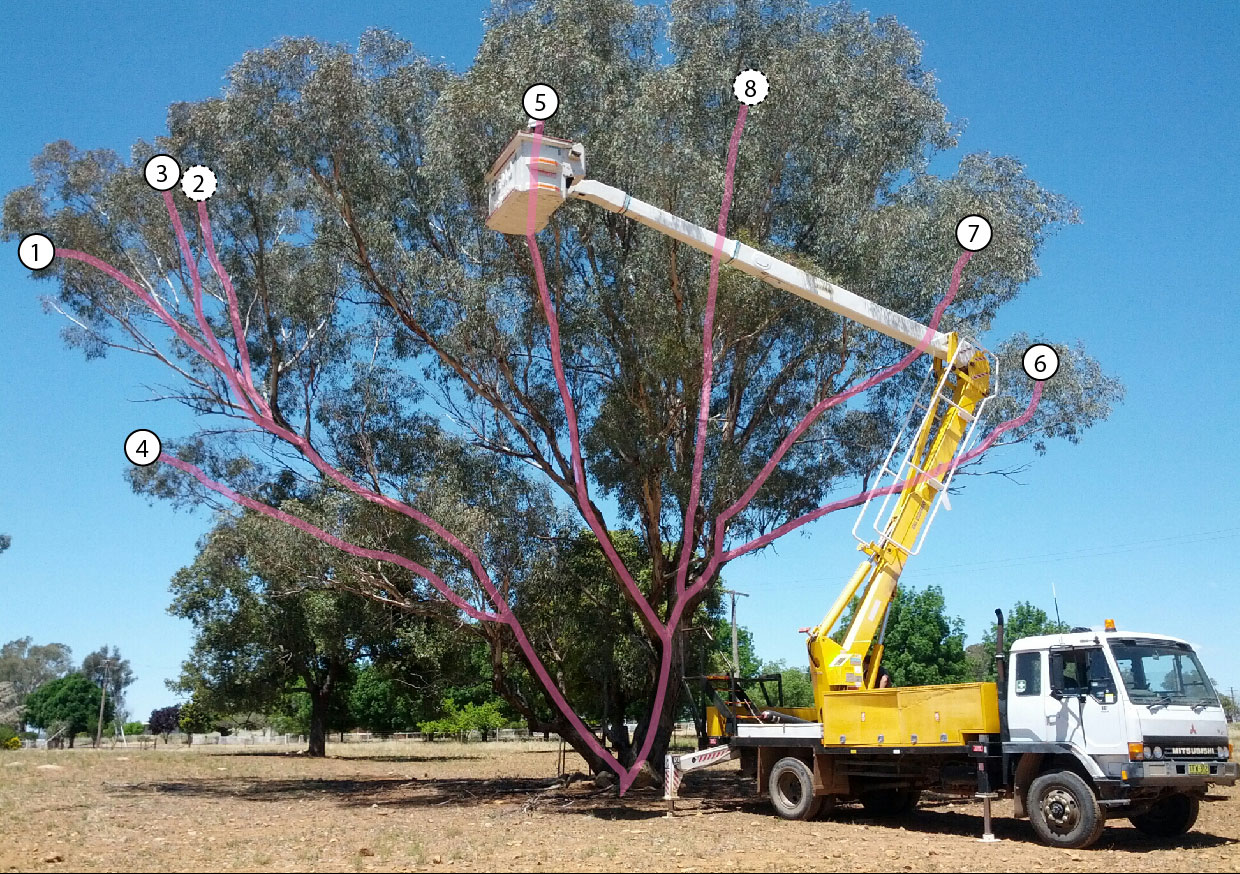
\includegraphics[width=\linewidth]{labeled_tree.jpg}
% 	\end{columns}
% \end{frame}

% \begin{frame}{Branch 7}
% Branch 7 is consistently in the wrong place. Why? What's going on with that branch?
% \begin{definition}
% 	\textbf{Long Branch Attraction} is the tendency of long branches to cluster in a phylogenetic tree
% \end{definition}

% \begin{itemize}
% \item Branch 7 is the longest branch
% \item May be affected by assumptions about zygosity
% \item Do particular genomic regions make mutation calling more difficult for one method?
% \end{itemize}
% \end{frame}

\begin{frame}{If you want something done right...}

Use \textit{E. melliodora} genome as a starting place, then generate a new reference and map to that reference.

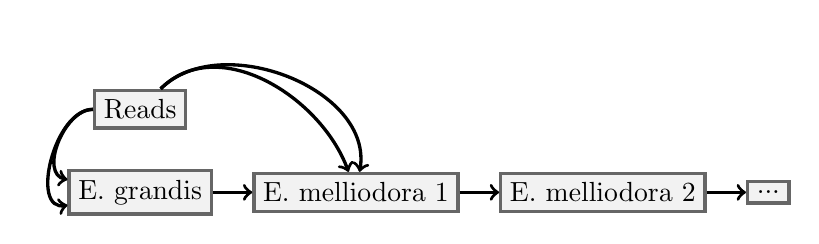
\begin{tikzpicture}[cnode/.style={rectangle,draw=black!60,fill=black!5,very thick}, node distance = .5 cm]
	\node[cnode] (reads){Reads};
	\node[cnode] (eg)[below = of reads]{E. grandis};
	\node[cnode] (em1)[right = of eg]{E. melliodora 1};
	\node[cnode] (em2)[right = of em1]{E. melliodora 2};
	\node[cnode] (etc)[right = of em2] {...};
	\draw[very thick,->] (reads) to [out=180,in=190] (eg);
	\draw[very thick,->] (reads) to [out=180,in=170] (eg);
	\draw[very thick,->] (reads) to [in=80] (em1);
	\draw[very thick,->] (reads) to [in=110] (em1);
	\draw[very thick,->] (eg) -- (em1);
	\draw[very thick,->] (em1) -- (em2);
	\draw[very thick,->] (em2) -- (etc);
\end{tikzpicture}

% \begin{alertblock}{Next Steps}
% \begin{itemize}
% \item Generate a genome and recursively improve it with multiple tools
% \item Filter repetitive elements that complicate mapping
% \item How do the mutations found with DiscoSNP compare to those found with GATK? Is there a pattern?
% \item Validation
% \end{itemize}
% \end{alertblock}

\end{frame}

\begin{frame}{Our New Reference Improves Mapping Quality}
\begin{center}
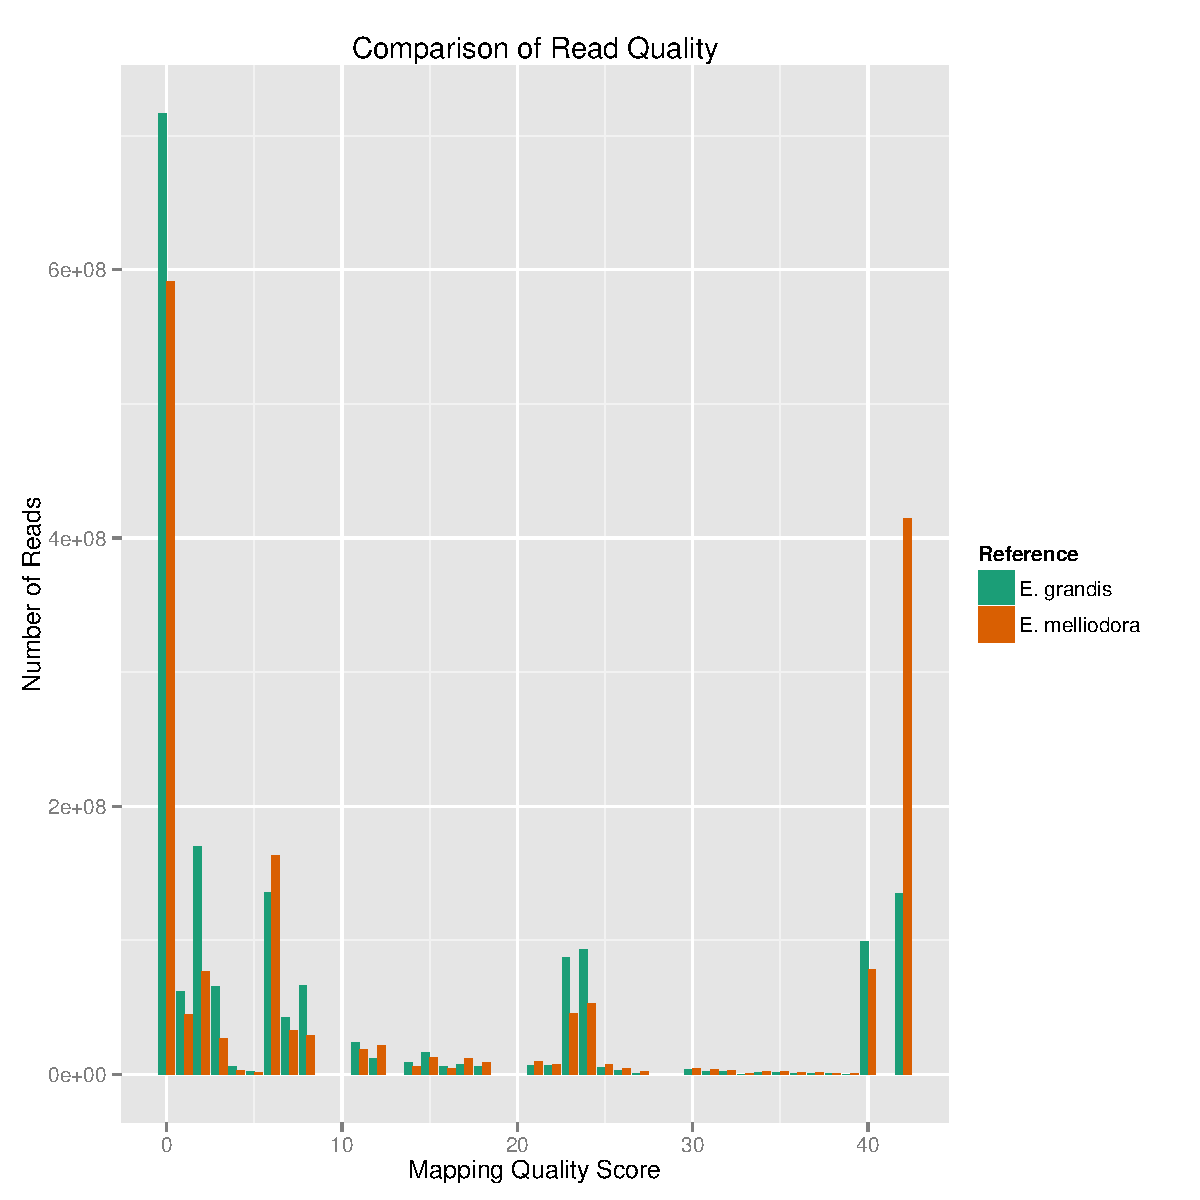
\includegraphics[width=.95\linewidth]{both_hist.pdf}
\end{center}
\end{frame}

\begin{frame}{The Choice of Aligner Impacts Mapping Quality}
\begin{center}
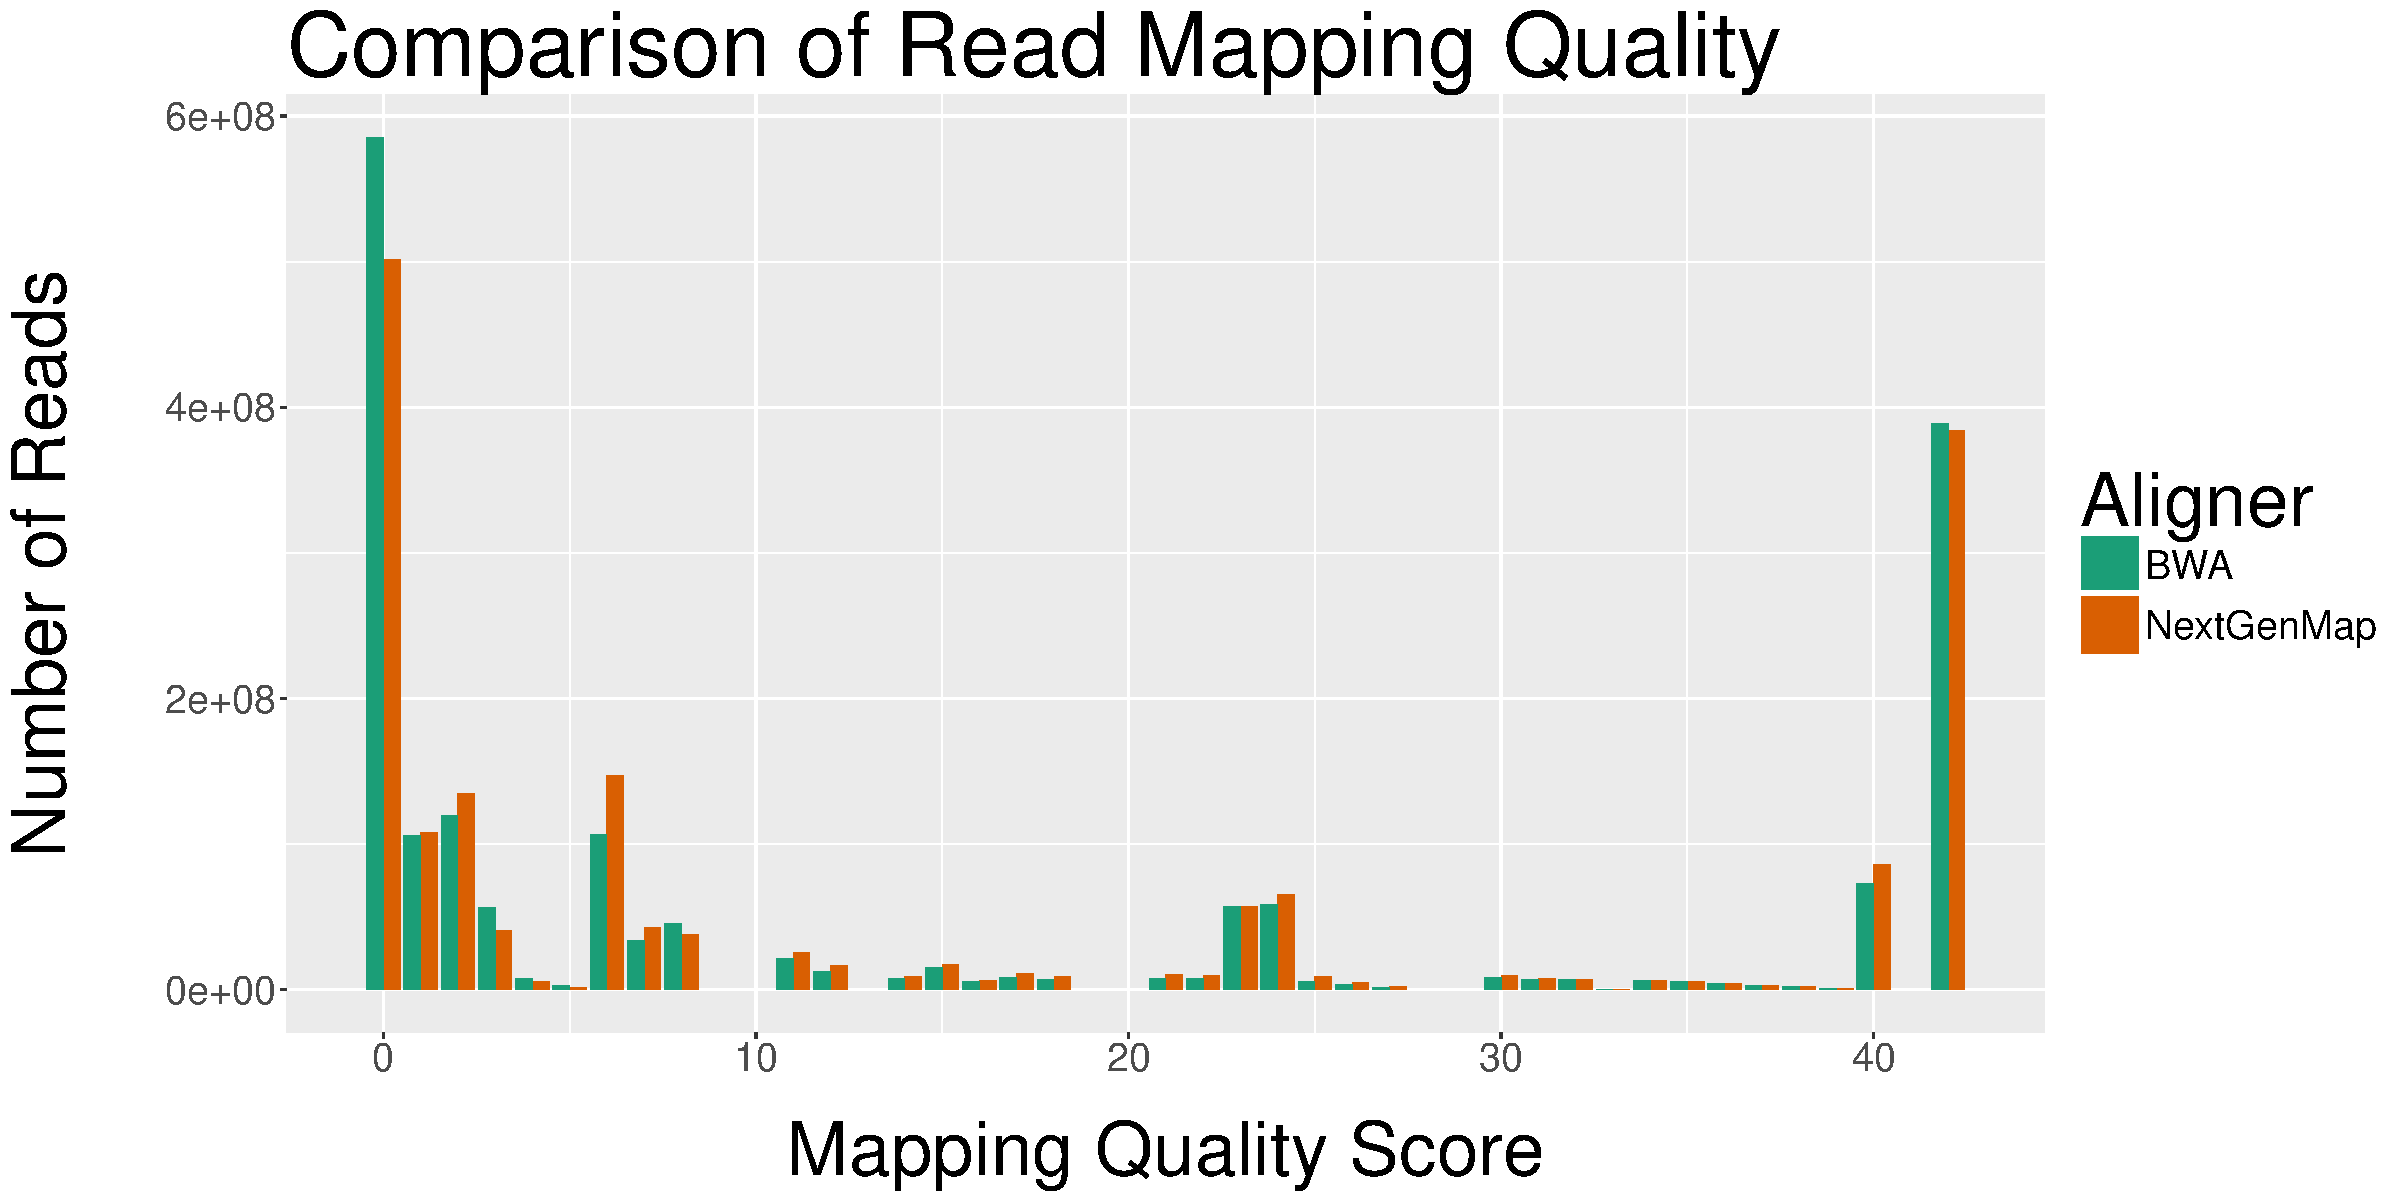
\includegraphics[width=.95\linewidth]{aligner_comparison_hist.pdf}
\end{center}
\end{frame}



\begin{frame}{Next Steps}
\begin{itemize}
\item Iterate to improve the reference we've created.
\item Filter out repetitive elements that make mapping difficult
\item Once we are confident in our results, make a prediction about the herbivore resistance
\item Validate
\end{itemize}
\end{frame}

\begin{frame}{Conclusions}
\begin{itemize}
\item A reference-free method performs similarly to a standard pipeline
\item Aligning to a reference, then using that alignment as a reference for another alignment can improve mapping qualities.
\item The choice of aligner can be important, especially if you are mapping to a divergent reference
\end{itemize}
\end{frame}

\begin{frame}{Acknowledgements}
\begin{itemize}
\item Reed Cartwright
\item Human and Comparative Genomics Laboratory
\item Robert Lanfear, Australian National University
\end{itemize}

\begin{columns}
\column{.4\linewidth}
	
\includegraphics[width=.9\linewidth]{lab_logo.pdf}
	\\~\\
	
\includegraphics[width=.9\linewidth]{biodesign_logo.pdf}
\column{.4\linewidth}
	
\includegraphics[width=.9\linewidth]{sols_logo.pdf}
	\\~\\
	
\includegraphics[width=.9\linewidth]{nih-nhgri-official-logo.jpg}
\end{columns}

\end{frame}

%Graph Theory
%How does a reference free method work?
%The tree I got
%Compare to GATK
%Why is this happening? IDK
%Talk about improving the assembly

\end{document}